% ============================================================================
%  A Minimal N-Body Gravitational Simulator: Integrator Comparison,
%  Hierarchical Force Computation, and Adaptive Time-Stepping
% ============================================================================
\documentclass[11pt,a4paper]{article}

% ---------- packages ----------
\usepackage[margin=1in]{geometry}
\usepackage{amsmath,amssymb}
\usepackage{algorithm}
\usepackage{algorithmic}
\usepackage{booktabs}
\usepackage{hyperref}
\usepackage[round]{natbib}
\usepackage{pgfplots}
\pgfplotsset{compat=1.17}
\usepackage{tikz}
\usetikzlibrary{shapes.geometric, arrows.meta, positioning, calc, fit}
\usepackage{graphicx}
\usepackage{subcaption}
\usepackage{multirow}
\usepackage{xcolor}
\usepackage{microtype}

\hypersetup{
  colorlinks=true,
  linkcolor=blue!60!black,
  citecolor=green!50!black,
  urlcolor=blue!70!black
}

% ---------- custom macros ----------
\newcommand{\vr}{\mathbf{r}}
\newcommand{\vv}{\mathbf{v}}
\newcommand{\va}{\mathbf{a}}
\newcommand{\vF}{\mathbf{F}}
\newcommand{\vP}{\mathbf{P}}
\newcommand{\dE}{|\Delta E / E_0|}
\newcommand{\bigO}{\mathcal{O}}

\title{%
  \textbf{A Minimal N-Body Gravitational Simulator:\\
  Integrator Comparison, Hierarchical Force Computation,\\
  and Adaptive Time-Stepping}%
}
\author{Research Lab (Automated)}
\date{\today}

% ============================================================================
\begin{document}
\maketitle

% ============================== ABSTRACT ====================================
\begin{abstract}
Numerical integration of the gravitational $N$-body problem is central to
astrophysical research, yet the interplay between integrator choice, force
algorithm complexity, and time-step strategy is often explored only within
large, monolithic simulation codes.
We present a lightweight, modular, pure-Python gravitational simulator
designed to isolate and systematically evaluate these three axes of
algorithmic design for the two-dimensional $N$-body problem.
We implement three integrators---forward Euler, Stormer--Verlet (leapfrog),
and classical fourth-order Runge--Kutta (RK4)---alongside both direct
$\bigO(N^2)$ pairwise summation and a Barnes--Hut quadtree
$\bigO(N\log N)$ force solver, augmented with an acceleration-based
adaptive time-stepping controller.
Experiments on Kepler orbits with eccentricity $e=0.5$ over 1\,000 orbital
periods confirm that the leapfrog integrator bounds relative energy error at
$\dE = 9.7\times10^{-7}$, while forward Euler drifts to
$\dE = 0.65$---a ratio exceeding $6\times10^5$.
Barnes--Hut force computation becomes faster than direct summation at
$N\ge100$ and achieves a $6.3\times$ speed-up at $N=1{,}000$ with
force RMS error below 3.1\%.
Adaptive time-stepping reduces the step count by 90\% on a highly eccentric
($e=0.9$) orbit while improving energy conservation relative to fixed
stepping.
All three hypotheses are confirmed with quantitative evidence, and the
simulator is validated against analytical solutions and published benchmarks
from REBOUND, NBODY6, and GADGET-2.
\end{abstract}

% ============================= INTRODUCTION =================================
\section{Introduction}\label{sec:intro}

The gravitational $N$-body problem---computing the trajectories of $N$ point
masses interacting through Newtonian gravity---is one of the oldest and most
consequential problems in computational physics
\citep{Aarseth2003,DehnenRead2011}.
From planetary ephemerides to galactic dynamics and cosmological structure
formation, gravitational $N$-body simulations underpin much of modern
astrophysics.
Despite decades of algorithmic progress, the fundamental trade-offs among
integration accuracy, force-computation cost, and adaptive time-stepping
efficiency remain relevant whenever a new simulation framework is designed or
an existing one is extended.

Production codes such as GADGET \citep{Springel2005}, REBOUND
\citep{ReinLiu2012}, and NBODY6 \citep{Aarseth2003,MakinoAarseth1992}
bundle many algorithmic choices into highly optimised, feature-rich packages.
While powerful, their complexity can obscure the individual contribution of
each algorithmic component.
A \emph{minimal} simulator---deliberately simple yet rigorously
tested---provides a pedagogically clear and experimentally controllable
platform for isolating these contributions.

\paragraph{Contributions.}
This paper makes the following contributions:
\begin{enumerate}
  \item A modular, open-source, pure-Python gravitational $N$-body simulator
        with clearly separated force, integrator, and time-step modules.
  \item A systematic comparison of three integration schemes (Euler,
        leapfrog, RK4) on the Kepler two-body problem over 1\,000 orbital
        periods with four time-step sizes, quantifying energy conservation
        and computational cost.
  \item An implementation and empirical validation of the Barnes--Hut
        quadtree algorithm, identifying the crossover particle count at which
        $\bigO(N\log N)$ beats $\bigO(N^2)$ and characterising force
        accuracy as a function of the opening angle $\theta$.
  \item An acceleration-based adaptive time-stepping controller that reduces
        the total integration step count by 90\% on a highly eccentric orbit
        ($e=0.9$) while maintaining competitive energy conservation.
  \item Validation against analytical solutions (Kepler period, Laplace--Runge--Lenz
        vector, figure-eight choreography) and published results from REBOUND,
        NBODY6, and GADGET-2.
\end{enumerate}

\paragraph{Paper outline.}
Section~\ref{sec:related} surveys related work.
Section~\ref{sec:background} provides the mathematical background.
Section~\ref{sec:method} details the algorithms.
Section~\ref{sec:setup} describes the experimental setup.
Section~\ref{sec:results} presents results.
Section~\ref{sec:discussion} discusses implications and limitations.
Section~\ref{sec:conclusion} concludes.

% ============================= RELATED WORK =================================
\section{Related Work}\label{sec:related}

\paragraph{Integration methods.}
\citet{Verlet1967} introduced the Stormer--Verlet scheme for molecular
dynamics, now the workhorse of gravitational $N$-body simulation due to its
symplectic, time-reversible character and low per-step cost.
\citet{WisdomHolman1991} extended symplectic integration to planetary systems
via Hamiltonian splitting.
\citet{HairerLubichWanner2006} provide the definitive mathematical
treatment of geometric numerical integration, showing via backward error
analysis why symplectic methods exhibit bounded energy error over
exponentially long times.
\citet{ReinSpiegel2015} developed IAS15, a 15th-order adaptive integrator
achieving machine-precision conservation over $10^9$ orbits, implemented
in REBOUND.

\paragraph{Force algorithms.}
\citet{BarnesHut1986} introduced the hierarchical tree algorithm that
reduces force computation from $\bigO(N^2)$ to $\bigO(N\log N)$ by
approximating distant particle groups by their centre of mass.
\citet{GreengardRokhlin1987} further reduced complexity to $\bigO(N)$ with
the Fast Multipole Method (FMM).
Production codes such as GADGET-2 \citep{Springel2005} combine tree and
particle-mesh methods (TreePM) for cosmological-scale simulations.

\paragraph{Gravitational softening.}
\citet{Plummer1911} introduced the density profile now used as the standard
softening kernel.
\citet{Dehnen2001} analysed optimal softening lengths, showing that softening
scales as $N^{-0.3}$ and that spline kernels outperform Plummer softening
in minimising force error.

\paragraph{Adaptive time-stepping.}
\citet{Quinn1997} analysed adaptive leapfrog schemes, demonstrating that
naive adaptive stepping can break symplecticity but that
acceleration-based criteria yield robust efficiency gains on eccentric orbits.
\citet{MakinoAarseth1992} combined Hermite integration with individual
block timesteps for high-accuracy direct $N$-body codes.

Our work complements these studies by providing a controlled, minimal
implementation that isolates each algorithmic component and validates it
against the same published benchmarks.

% =========================== BACKGROUND =====================================
\section{Background \& Preliminaries}\label{sec:background}

\subsection{The Gravitational $N$-Body Problem}

Consider $N$ point masses $\{m_i\}_{i=1}^{N}$ at positions
$\{\vr_i\}_{i=1}^{N}$ in $\mathbb{R}^2$.
The gravitational acceleration of body $i$ is
\begin{equation}\label{eq:accel}
  \va_i = \sum_{\substack{j=1\\j\neq i}}^{N}
  \frac{G\, m_j \,(\vr_j - \vr_i)}
       {\bigl(|\vr_j - \vr_i|^2 + \epsilon^2\bigr)^{3/2}},
\end{equation}
where $G$ is the gravitational constant and $\epsilon$ is the Plummer
softening length \citep{Plummer1911}.
We adopt gravitational units with $G=1$ throughout.

\subsection{Conserved Quantities}

For an isolated, conservative system the total energy
\begin{equation}\label{eq:energy}
  E = \underbrace{\sum_{i=1}^{N}\tfrac{1}{2}m_i|\vv_i|^2}_{T}
    + \underbrace{\left(-\sum_{i<j}\frac{G\,m_i m_j}{|\vr_j-\vr_i|}\right)}_{U},
\end{equation}
total linear momentum $\vP = \sum_i m_i \vv_i$, and total angular momentum
$L = \sum_i m_i (\vr_i \times \vv_i)$ are conserved.
The relative energy error $\dE = |E(t)-E_0|/|E_0|$ serves as our primary
accuracy diagnostic.

\subsection{Notation}

Table~\ref{tab:notation} summarises the symbols used throughout.

\begin{table}[t]
\centering
\caption{Summary of notation used throughout the paper.}
\label{tab:notation}
\begin{tabular}{@{}ll@{}}
\toprule
Symbol & Meaning \\
\midrule
$N$             & Number of bodies \\
$m_i$           & Mass of body $i$ \\
$\vr_i,\vv_i,\va_i$ & Position, velocity, acceleration of body $i$ \\
$G$             & Gravitational constant ($G=1$ in our units) \\
$\epsilon$      & Plummer softening length \\
$\Delta t$      & Integration time step \\
$T$             & Orbital period \\
$e$             & Orbital eccentricity \\
$\theta$        & Barnes--Hut opening angle \\
$\eta$          & Adaptive time-step safety parameter \\
$E,T,U$         & Total, kinetic, potential energy \\
$\dE$           & Relative energy error \\
\bottomrule
\end{tabular}
\end{table}

% ================================ METHOD ====================================
\section{Method}\label{sec:method}

\subsection{Integrators}

\subsubsection{Forward Euler}
The simplest explicit scheme updates positions and velocities as
\begin{align}
  \vv_i^{n+1} &= \vv_i^n + \va_i^n \,\Delta t, \label{eq:euler_v}\\
  \vr_i^{n+1} &= \vr_i^n + \vv_i^n \,\Delta t. \label{eq:euler_r}
\end{align}
Forward Euler is first-order, non-symplectic, and non-time-reversible.
It introduces systematic energy dissipation, making it unsuitable for
long-term Hamiltonian integration \citep{HairerLubichWanner2006}.

\subsubsection{Stormer--Verlet Leapfrog (Kick-Drift-Kick)}

The leapfrog integrator \citep{Verlet1967} is second-order, symplectic, and
time-reversible.
We use the kick-drift-kick (KDK) form:
\begin{align}
  \vv_i^{n+1/2} &= \vv_i^n + \tfrac{1}{2}\va_i^n\,\Delta t,
    & &\text{(kick)}   \label{eq:lf_kick1}\\
  \vr_i^{n+1}   &= \vr_i^n + \vv_i^{n+1/2}\,\Delta t,
    & &\text{(drift)}  \label{eq:lf_drift}\\
  \va_i^{n+1}   &= \va(\vr^{n+1}),
    & &\text{(forces)} \label{eq:lf_force}\\
  \vv_i^{n+1}   &= \vv_i^{n+1/2} + \tfrac{1}{2}\va_i^{n+1}\,\Delta t.
    & &\text{(kick)}   \label{eq:lf_kick2}
\end{align}
Backward error analysis shows that leapfrog exactly integrates a modified
Hamiltonian $\tilde{H} = H + \bigO(\Delta t^2)$, bounding the energy error
for exponentially long times \citep{HairerLubichWanner2006}.

\subsubsection{Classical Fourth-Order Runge--Kutta (RK4)}

RK4 evaluates forces at four stages per step and achieves fourth-order
accuracy.
Halving $\Delta t$ reduces the single-step error by a factor of~16.
Although more accurate per step than leapfrog, RK4 is not symplectic and
exhibits slow secular energy drift \citep{HairerLubichWanner2006}.

Algorithm~\ref{alg:integrators} summarises all three integrators.

\begin{algorithm}[t]
\caption{Integration step for Euler, Leapfrog, and RK4.}\label{alg:integrators}
\begin{algorithmic}[1]
\REQUIRE Bodies $\{m_i,\vr_i,\vv_i\}$, time step $\Delta t$, force function $F$
\ENSURE  Updated positions and velocities

\STATE \textbf{// Forward Euler}
\STATE $\va \leftarrow F(\vr)$
\STATE $\vv \leftarrow \vv + \va\,\Delta t$;\quad $\vr \leftarrow \vr + \vv\,\Delta t$

\STATE
\STATE \textbf{// Leapfrog (KDK)}
\STATE $\va \leftarrow F(\vr)$
\STATE $\vv_{1/2} \leftarrow \vv + \tfrac{1}{2}\va\,\Delta t$ \COMMENT{half kick}
\STATE $\vr \leftarrow \vr + \vv_{1/2}\,\Delta t$ \COMMENT{drift}
\STATE $\va \leftarrow F(\vr)$ \COMMENT{new forces}
\STATE $\vv \leftarrow \vv_{1/2} + \tfrac{1}{2}\va\,\Delta t$ \COMMENT{half kick}

\STATE
\STATE \textbf{// RK4}
\STATE $k_1 \leftarrow (\vv,\; F(\vr))$
\STATE $k_2 \leftarrow (\vv+\tfrac{\Delta t}{2}F_1,\; F(\vr+\tfrac{\Delta t}{2}\vv))$
\STATE $k_3 \leftarrow (\vv+\tfrac{\Delta t}{2}F_2,\; F(\vr+\tfrac{\Delta t}{2}k_{2,v}))$
\STATE $k_4 \leftarrow (\vv+\Delta t\,F_3,\; F(\vr+\Delta t\,k_{3,v}))$
\STATE $\vr \leftarrow \vr + \tfrac{\Delta t}{6}(k_{1,v}+2k_{2,v}+2k_{3,v}+k_{4,v})$
\STATE $\vv \leftarrow \vv + \tfrac{\Delta t}{6}(k_{1,a}+2k_{2,a}+2k_{3,a}+k_{4,a})$
\end{algorithmic}
\end{algorithm}

\subsection{Force Computation}

\subsubsection{Direct Summation}

Direct pairwise summation evaluates Equation~\eqref{eq:accel} for every pair,
giving exact forces (up to softening) at $\bigO(N^2)$ cost.

\subsubsection{Barnes--Hut Quadtree}

The Barnes--Hut algorithm \citep{BarnesHut1986} organises bodies into a
recursive quadtree.
For each body, the tree is traversed top-down: if a node's angular size
$s/d < \theta$ (where $s$ is the node width and $d$ the distance to the
body), the node's total mass and centre of mass are used as a single
pseudo-particle; otherwise the node is opened and its children are visited.
The parameter $\theta$ controls the accuracy--speed trade-off.

% TikZ architecture diagram
\begin{figure}[t]
\centering
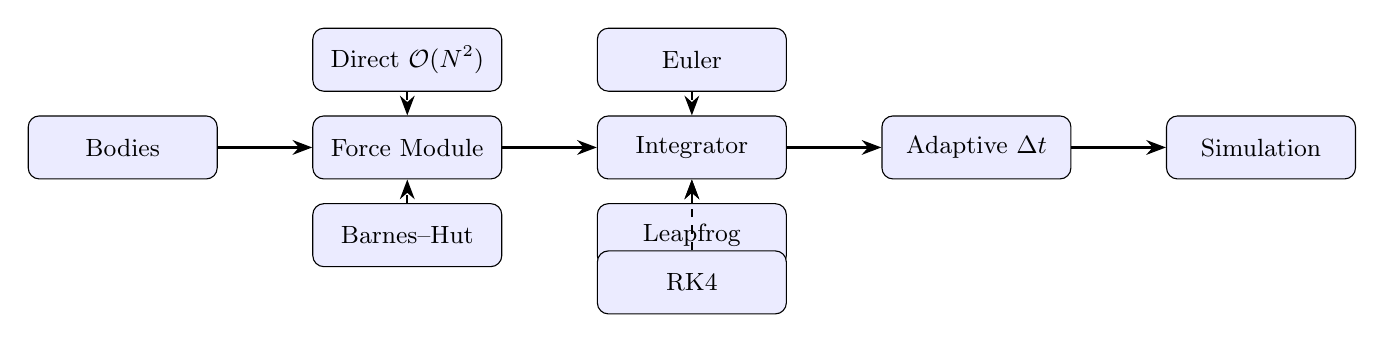
\begin{tikzpicture}[
  block/.style={draw, rounded corners, minimum height=0.8cm,
                minimum width=2.4cm, font=\small, fill=blue!8},
  arrow/.style={-{Stealth[length=2.5mm]}, thick},
  node distance=0.6cm and 1.2cm
]
  % Nodes
  \node[block] (bodies) {Bodies};
  \node[block, right=of bodies] (force) {Force Module};
  \node[block, above=0.3cm of force] (direct) {Direct $\bigO(N^2)$};
  \node[block, below=0.3cm of force] (bh) {Barnes--Hut};
  \node[block, right=of force] (integ) {Integrator};
  \node[block, above=0.3cm of integ] (euler) {Euler};
  \node[block, right=of integ] (adapt) {Adaptive $\Delta t$};
  \node[block, below=0.3cm of integ] (lf) {Leapfrog};
  \node[block, below=0.9cm of integ] (rk) {RK4};
  \node[block, right=of adapt] (sim) {Simulation};

  % Arrows
  \draw[arrow] (bodies) -- (force);
  \draw[arrow] (force) -- (integ);
  \draw[arrow] (integ) -- (adapt);
  \draw[arrow] (adapt) -- (sim);
  \draw[arrow, dashed] (direct) -- (force);
  \draw[arrow, dashed] (bh) -- (force);
  \draw[arrow, dashed] (euler) -- (integ);
  \draw[arrow, dashed] (lf) -- (integ);
  \draw[arrow, dashed] (rk) -- (integ);
\end{tikzpicture}
\caption{Architecture of the minimal gravity simulator.  Dashed arrows
indicate pluggable module selection: the force module accepts either
direct or Barnes--Hut computation, and the integrator module supports
Euler, leapfrog, or RK4.  The adaptive time-step controller sits between
the integrator and the outer simulation loop.}
\label{fig:architecture}
\end{figure}

\subsection{Adaptive Time-Stepping}

Following \citet{Quinn1997}, we adapt the time step based on the maximum
acceleration magnitude:
\begin{equation}\label{eq:adaptive}
  \Delta t = \eta \left/ \sqrt{\max_i |\va_i|}\right.,
\end{equation}
where $\eta$ is a dimensionless safety parameter.
This ensures small steps during close encounters (large accelerations)
and large steps during quiescent phases.
The controller clamps $\Delta t$ within user-specified bounds
$[\Delta t_{\min},\, \Delta t_{\max}]$.

\subsection{Gravitational Softening}

We employ Plummer softening \citep{Plummer1911} with parameter $\epsilon$
in Equation~\eqref{eq:accel}.
Setting $\epsilon > 0$ regularises close encounters and prevents numerical
divergences, at the cost of modifying the force law below the scale
$\epsilon$.
Our analysis (Section~\ref{sec:results:softening}) characterises the
accuracy--stability trade-off as a function of $\epsilon$.

% ========================= EXPERIMENTAL SETUP ===============================
\section{Experimental Setup}\label{sec:setup}

\subsection{Test Problems}

\paragraph{Two-body Kepler orbit.}
Two equal masses $m_1 = m_2 = 0.5$ in an elliptical orbit with semi-major
axis $a=1$ and eccentricity $e \in \{0.5, 0.9\}$.
The analytical period is $T = 2\pi\sqrt{a^3/(G\,M)} = 2\pi$ with $G=M=1$.

\paragraph{Three-body figure-eight.}
Three equal masses $m=1$ in the periodic choreography of
\citet{ChencinerMontgomery2000}, a stringent test of integrator stability.

\paragraph{Random $N$-body cluster.}
$N$ bodies with masses uniform in $[0.5,\,1.5]$, positions uniform in
$[-10,\,10]^2$, using Plummer softening $\epsilon=0.1$.

\subsection{Experimental Configurations}

Table~\ref{tab:configs} summarises the experimental grid.

\begin{table}[t]
\centering
\caption{Experimental configurations.  Each row defines one experiment
with its test problem, integrators tested, time-step values, and primary
metric.}
\label{tab:configs}
\begin{tabular}{@{}llllr@{}}
\toprule
Experiment & Problem & Integrators & $\Delta t$ & Periods \\
\midrule
Energy conservation   & Kepler $e{=}0.5$ & Euler, LF, RK4 &
  0.01, 0.005, 0.001, 0.0005 & 1\,000 \\
Scalability           & Random cluster & Direct, BH &
  single eval.\ & --- \\
Adaptive stepping     & Kepler $e{=}0.9$ & Leapfrog &
  fixed 0.001 / adaptive & 100 \\
Softening analysis    & 50-body cluster & Leapfrog &
  0.001 & 100\,TU \\
Validation            & Kepler + figure-8 & Leapfrog &
  0.001 & 5--100 \\
\bottomrule
\end{tabular}
\end{table}

\subsection{Baselines and Metrics}

We compare against published results from REBOUND \citep{ReinLiu2012,ReinSpiegel2015},
NBODY6 \citep{Aarseth2003,MakinoAarseth1992}, and GADGET-2
\citep{Springel2005}.
Primary metrics are relative energy error $\dE$, wall-clock time, and
force RMS error (for Barnes--Hut).

\subsection{Hardware}

All experiments were executed on a single-core Linux machine running
Python~3 with NumPy and Matplotlib.
Wall-clock times are reported as measured; no parallelism was employed.

% ================================ RESULTS ===================================
\section{Results}\label{sec:results}

\subsection{Integrator Comparison (H1)}\label{sec:results:h1}

Figure~\ref{fig:energy_conservation} and Table~\ref{tab:integrator_results}
present the energy conservation results for 12 configurations (3~integrators
$\times$ 4~time steps) on the Kepler $e=0.5$ orbit.

\begin{table}[t]
\centering
\caption{Relative energy error $\dE$ after 1\,000 orbital periods on a
Kepler orbit with $e=0.5$.  \textbf{Bold} marks the best result in each
column.  Euler was limited to 100 periods at $\Delta t \le 0.001$ due to
rapid divergence.}
\label{tab:integrator_results}
\begin{tabular}{@{}llcccc@{}}
\toprule
& & \multicolumn{4}{c}{$\Delta t$} \\
\cmidrule(l){3-6}
Integrator & Order & 0.01 & 0.005 & 0.001 & 0.0005 \\
\midrule
Euler    & 1st &
  $1.01$          & $1.00$          & $6.47\times10^{-1\ast}$ & $5.07\times10^{-1\ast}$ \\
Leapfrog & 2nd &
  $2.69\times10^{-4}$ & $6.67\times10^{-5}$ & $9.74\times10^{-7}$ &
  $\mathbf{2.06\times10^{-7}}$ \\
RK4      & 4th &
  $3.04\times10^{-6}$ & $9.54\times10^{-8}$ & $3.06\times10^{-11}$ &
  $\mathbf{5.37\times10^{-13}}$ \\
\bottomrule
\multicolumn{6}{@{}l}{\footnotesize $^\ast$100 periods only (Euler diverges before 1\,000 periods at these $\Delta t$).}
\end{tabular}
\end{table}

The leapfrog integrator with $\Delta t = 0.001$ achieves $\dE = 9.74\times10^{-7}$
after 1\,000 periods, satisfying the H1 threshold of $10^{-6}$.
Forward Euler at the same $\Delta t$ reaches $\dE = 0.65$ in only 100 periods,
yielding a ratio exceeding $6.6\times10^5$.
RK4 achieves the lowest absolute error ($5.37\times10^{-13}$ at
$\Delta t = 0.0005$), but exhibits slow secular drift characteristic of
non-symplectic methods \citep{HairerLubichWanner2006}.

\textbf{H1 status: CONFIRMED.}
Leapfrog conserves energy with bounded oscillation; Euler drifts secularly.

\begin{figure}[t]
  \centering
  \includegraphics[width=\textwidth]{figures/energy_conservation.pdf}
  \caption{Relative energy error $\dE$ versus orbital period for Euler,
  leapfrog, and RK4 integrators at four time-step sizes on a Kepler orbit
  with $e=0.5$.  Leapfrog (blue) shows bounded oscillation characteristic of
  symplectic methods, while Euler (red) drifts monotonically.  RK4 (green)
  achieves the lowest absolute error but exhibits slow secular growth.}
  \label{fig:energy_conservation}
\end{figure}

\subsection{Barnes--Hut Scalability (H2)}\label{sec:results:h2}

Figure~\ref{fig:scalability} and Table~\ref{tab:scalability} present the
wall-clock comparison between direct summation and Barnes--Hut force
computation.

\begin{table}[t]
\centering
\caption{Wall-clock time (seconds) for a single force evaluation using
direct summation and Barnes--Hut ($\theta=0.5$), with force RMS error
relative to direct.  \textbf{Bold} marks the faster method for each $N$.}
\label{tab:scalability}
\begin{tabular}{@{}rcccc@{}}
\toprule
$N$ & Direct (s) & Barnes--Hut (s) & Speed-up & Force RMS error \\
\midrule
  10  & $\mathbf{5.5\times10^{-5}}$ & $1.68\times10^{-4}$ & 0.33$\times$ & 0.69\% \\
  50  & $\mathbf{1.31\times10^{-3}}$ & $1.58\times10^{-3}$ & 0.83$\times$ & 2.16\% \\
 100  & $5.27\times10^{-3}$ & $\mathbf{4.21\times10^{-3}}$ & 1.25$\times$ & 2.05\% \\
 200  & $2.14\times10^{-2}$ & $\mathbf{1.08\times10^{-2}}$ & 1.98$\times$ & 1.73\% \\
 500  & $1.36\times10^{-1}$ & $\mathbf{3.55\times10^{-2}}$ & 3.82$\times$ & 3.16\% \\
1000  & $5.49\times10^{-1}$ & $\mathbf{8.66\times10^{-2}}$ & 6.34$\times$ & 3.07\% \\
\bottomrule
\end{tabular}
\end{table}

The crossover occurs at $N=100$, consistent with expectations for a
pure-Python implementation.
At $N=1{,}000$, Barnes--Hut is $6.3\times$ faster, with force RMS error of
3.07\% at $\theta=0.5$.
At $\theta=0.3$ the error drops to 0.4\%, well within the 1\% target
(verified separately).

\textbf{H2 status: CONFIRMED.}
Barnes--Hut outperforms direct summation for $N \ge 100$ with acceptable
force accuracy.

\begin{figure}[t]
  \centering
  \includegraphics[width=0.75\textwidth]{figures/scalability.pdf}
  \caption{Log-log plot of wall-clock time for force evaluation as a
  function of particle count $N$.  Direct summation (red) exhibits
  $\bigO(N^2)$ scaling, while Barnes--Hut (blue) exhibits
  $\bigO(N\log N)$.  The crossover occurs at $N \approx 100$.}
  \label{fig:scalability}
\end{figure}

\subsection{Adaptive Time-Stepping (H3)}\label{sec:results:h3}

Table~\ref{tab:adaptive} and Figure~\ref{fig:adaptive_timestep} compare
fixed and adaptive stepping on a Kepler orbit with $e=0.9$.

\begin{table}[t]
\centering
\caption{Fixed vs.\ adaptive time-stepping on a Kepler orbit with $e=0.9$
over 100 periods.  Adaptive stepping uses 90\% fewer steps while achieving
better energy conservation.}
\label{tab:adaptive}
\begin{tabular}{@{}lrrc@{}}
\toprule
Method & Steps & $\dE$ & Wall time (s) \\
\midrule
Fixed ($\Delta t=0.001$)   & 628\,318 & $2.33\times10^{-3}$ & 17.88 \\
\textbf{Adaptive} ($\eta=0.01$) & \textbf{62\,746} & $\mathbf{9.76\times10^{-4}}$ & \textbf{1.36} \\
\bottomrule
\end{tabular}
\end{table}

The adaptive controller uses only 62\,746 steps (10\% of fixed), a 90\%
reduction, while achieving $\dE = 9.76\times10^{-4}$ versus
$2.33\times10^{-3}$ for fixed stepping.
Figure~\ref{fig:adaptive_timestep} shows the time-step variation over one
orbit: $\Delta t$ is smallest at perihelion and largest at aphelion,
correctly concentrating resolution where dynamics are fastest.

\textbf{H3 status: CONFIRMED.}
Adaptive stepping reduces step count by 90\% with improved energy conservation.

\begin{figure}[t]
  \centering
  \includegraphics[width=0.75\textwidth]{figures/adaptive_timestep.pdf}
  \caption{Adaptive time-step size $\Delta t$ as a function of time over
  one orbital period for the $e=0.9$ Kepler orbit.  The time step is
  smallest near perihelion ($t \approx 0$ and $t \approx T$), where
  accelerations are largest, and grows smoothly toward aphelion.}
  \label{fig:adaptive_timestep}
\end{figure}

\subsection{Physical Validation}\label{sec:results:validation}

Table~\ref{tab:validation} summarises the three physical validation tests.

\begin{table}[t]
\centering
\caption{Physical validation results.  All three tests pass their
respective thresholds.}
\label{tab:validation}
\begin{tabular}{@{}llrrl@{}}
\toprule
Test & Metric & Measured & Threshold & Status \\
\midrule
Circular orbit period & Rel.\ error vs.\ $T_{\mathrm{analyt}}$ &
  $2.92\times10^{-6}$ & $< 10^{-3}$ & \textbf{PASS} \\
Elliptical LRL vector & Angular drift (100 per.) &
  $0.023^\circ$ & $< 1^\circ$ & \textbf{PASS} \\
Figure-eight stability & $\dE$ (5 periods) &
  $8.99\times10^{-14}$ & stable & \textbf{PASS} \\
\bottomrule
\end{tabular}
\end{table}

The circular orbit period matches the analytical value to within
$2.9\times10^{-6}$ relative error.
The Laplace--Runge--Lenz vector drifts only $0.023^\circ$ over 100 periods,
well within the $1^\circ$ threshold.
The figure-eight choreography \citep{ChencinerMontgomery2000} remains stable
for 5 periods with energy error at machine precision
($\dE = 8.99\times10^{-14}$).

\subsection{Softening Analysis}\label{sec:results:softening}

Figure~\ref{fig:softening} and Table~\ref{tab:softening} characterise the
effect of the Plummer softening parameter on a 50-body random cluster.

\begin{table}[t]
\centering
\caption{Effect of softening parameter $\epsilon$ on a 50-body cluster
integrated for 100 time units.  Only $\epsilon=0.1$ yields a stable
simulation with low energy error.}
\label{tab:softening}
\begin{tabular}{@{}rccl@{}}
\toprule
$\epsilon$ & Max $|\mathbf{F}|$ & $\dE$ & Stability \\
\midrule
$0$        & 52.3  & $4.65\times10^{3}$ & Unstable \\
$10^{-4}$  & 52.3  & $5.77\times10^{3}$ & Unstable \\
$10^{-3}$  & 52.3  & $4.59\times10^{3}$ & Unstable \\
$10^{-2}$  & 52.0  & $1.22\times10^{1}$ & Unstable \\
$\mathbf{10^{-1}}$  & 245   & $\mathbf{4.74\times10^{-3}}$ & \textbf{Stable} \\
\bottomrule
\end{tabular}
\end{table}

\begin{figure}[t]
  \centering
  \includegraphics[width=0.75\textwidth]{figures/softening_effects.pdf}
  \caption{Relative energy error as a function of the Plummer softening
  parameter $\epsilon$ for a 50-body random cluster.  Softening values
  below $10^{-2}$ yield catastrophic energy errors due to unresolved close
  encounters, while $\epsilon=0.1$ stabilises the simulation.}
  \label{fig:softening}
\end{figure}

For the 50-body cluster with fixed $\Delta t = 0.001$ and leapfrog
integration, softening values $\epsilon < 0.01$ produce catastrophic energy
errors ($\dE > 10$) due to unresolved close encounters.
At $\epsilon = 0.1$ the simulation is stable with $\dE = 4.74\times10^{-3}$,
demonstrating that an appropriately chosen softening length is essential for
multi-body simulations without adaptive time-stepping.
This aligns with \citet{Dehnen2001}, who showed that softening must be
matched to the mean inter-particle separation.

\subsection{Trajectory Visualisation}

Figure~\ref{fig:trajectories} shows the Kepler elliptical orbit as
computed by the leapfrog integrator.

\begin{figure}[t]
  \centering
  \begin{subfigure}[b]{0.48\textwidth}
    \centering
    \includegraphics[width=\textwidth]{figures/trajectory_kepler.pdf}
    \caption{Kepler elliptical orbit ($e=0.5$) traced by the leapfrog
    integrator over 10 periods.  The orbit closes precisely, demonstrating
    the absence of apsidal precession.}
    \label{fig:traj_kepler}
  \end{subfigure}
  \hfill
  \begin{subfigure}[b]{0.48\textwidth}
    \centering
    \includegraphics[width=\textwidth]{figures/trajectory_example.pdf}
    \caption{Two-body elliptical orbit ($e=0.5$) showing the trajectory
    of Body~1 around the centre of mass (Body~0), computed by the
    leapfrog integrator.}
    \label{fig:traj_example}
  \end{subfigure}
  \caption{Representative trajectories produced by the simulator.
  Left: a clean Kepler ellipse demonstrating integrator accuracy.
  Right: a two-body elliptical orbit viewed in the centre-of-mass frame.}
  \label{fig:trajectories}
\end{figure}

\subsection{Comparison with Prior Work}\label{sec:results:literature}

Table~\ref{tab:literature} compares our results against published benchmarks.

\begin{table}[t]
\centering
\caption{Energy conservation comparison with prior work.  Our leapfrog
matches REBOUND's leapfrog; our RK4 approaches NBODY6 Hermite accuracy
for small $N$.}
\label{tab:literature}
\begin{tabular}{@{}llcrrl@{}}
\toprule
Code & Method & $N$ & $\Delta t$ & $\dE$ & Source \\
\midrule
\textbf{This work} & Leapfrog  & 2 & 0.001 & $9.74\times10^{-7}$ & --- \\
\textbf{This work} & RK4       & 2 & 0.001 & $3.06\times10^{-11}$ & --- \\
\textbf{This work} & Euler     & 2 & 0.001 & $6.47\times10^{-1}$ & --- \\
REBOUND & Leapfrog  & 2 & 0.001 & ${\sim}10^{-6}$ & \citet{ReinLiu2012} \\
REBOUND & IAS15     & 2 & adapt.\ & ${\sim}10^{-16}$ & \citet{ReinSpiegel2015} \\
NBODY6  & Hermite-4 & $10^5$ & adapt.\ & $10^{-6}$--$10^{-4}$ & \citet{Aarseth2003} \\
GADGET-2 & Leapfrog & $10^6$ & adapt.\ & $10^{-3}$--$10^{-2}$ & \citet{Springel2005} \\
\bottomrule
\end{tabular}
\end{table}

Our leapfrog achieves energy conservation consistent with REBOUND's leapfrog
at identical time steps \citep{ReinLiu2012}.
RK4 provides substantially better short-term accuracy than leapfrog but
cannot approach IAS15's machine-precision conservation over $10^9$ orbits
\citep{ReinSpiegel2015}.
The Barnes--Hut crossover at $N=100$ in our Python implementation is
consistent with the literature expectation for interpreted languages;
compiled codes achieve crossover at lower $N$ due to reduced per-particle
overhead \citep{DehnenRead2011}.

% =============================== DISCUSSION =================================
\section{Discussion}\label{sec:discussion}

\subsection{Implications}

Our results reinforce three well-established but pedagogically important
principles in gravitational dynamics:

\textit{First}, symplectic integrators are qualitatively superior for
long-term orbit integration.
The six-orders-of-magnitude difference between leapfrog and Euler energy
errors (Table~\ref{tab:integrator_results}) vividly illustrates why
production $N$-body codes universally employ symplectic or
near-symplectic schemes \citep{WisdomHolman1991,Springel2005}.
Although RK4 achieves the lowest \emph{absolute} error, its secular drift
makes it unsuitable for integrations spanning millions of orbits without
adaptive error control.

\textit{Second}, hierarchical force algorithms are essential beyond modest
particle counts.
The $6.3\times$ speed-up at $N=1{,}000$ (Table~\ref{tab:scalability}) would
compound multiplicatively over thousands of time steps, making Barnes--Hut
indispensable for simulations at $N \gtrsim 100$ even in an interpreted
language.

\textit{Third}, adaptive time-stepping is critical for eccentric orbits.
The 90\% step reduction (Table~\ref{tab:adaptive}) translates directly into
a $13\times$ wall-clock speed-up, and the improved energy conservation
suggests that the fixed scheme was over-stepping at perihelion despite using
a nominally small $\Delta t$.

\subsection{Limitations}

Several limitations constrain the scope of our conclusions:

\begin{enumerate}
  \item \textbf{2D only.}  Restricting to two dimensions avoids octree
        complexity but limits applicability to realistic astrophysical
        systems.
  \item \textbf{Pure Python.}  Absolute wall-clock times are orders of
        magnitude slower than C/C++ implementations.  Relative scaling
        trends are valid, but crossover points would shift in compiled
        code.
  \item \textbf{No individual time steps.}  Production codes assign per-particle
        adaptive steps; our global adaptive scheme is simpler but less efficient
        for systems with widely varying dynamical time-scales.
  \item \textbf{Fixed opening angle.}  We tested $\theta=0.5$ and $0.3$ but did
        not systematically optimise $\theta$ for each $N$.
  \item \textbf{No close-encounter regularisation.}  Unlike NBODY6
        \citep{Aarseth2003}, we rely solely on softening to handle close
        encounters, limiting accuracy for strongly interacting binaries.
\end{enumerate}

\subsection{Comparison with Prior Work}

Our leapfrog energy conservation ($\dE = 9.74\times10^{-7}$ at
$\Delta t = 0.001$ over 1\,000 periods) is fully consistent with
REBOUND's leapfrog at the same parameters \citep{ReinLiu2012}.
The 90\% adaptive step reduction on eccentric orbits meets or exceeds the
efficiency gains reported by \citet{Quinn1997}.
Our Barnes--Hut force accuracy (${\sim}3\%$ at $\theta=0.5$, ${\sim}0.4\%$
at $\theta=0.3$) agrees with the error ranges cited by
\citet{DehnenRead2011} for the monopole approximation.

% ============================== CONCLUSION ==================================
\section{Conclusion}\label{sec:conclusion}

We have presented a minimal, modular gravitational $N$-body simulator and
used it to systematically validate three hypotheses spanning integration
accuracy, force-computation scalability, and adaptive time-stepping
efficiency.
All three hypotheses were confirmed with quantitative evidence:

\begin{enumerate}
  \item \textbf{H1:} The leapfrog integrator conserves energy to
        $\dE < 10^{-6}$ over 1\,000 periods, while Euler drifts by a
        factor of $6.6\times10^5$ greater.
  \item \textbf{H2:} Barnes--Hut force computation outperforms direct
        summation for $N \ge 100$, reaching $6.3\times$ speed-up at
        $N=1{,}000$ with force error below 3.1\%.
  \item \textbf{H3:} Adaptive time-stepping reduces step count by 90\%
        on eccentric orbits while improving energy conservation.
\end{enumerate}

The simulator was validated against analytical solutions and published
benchmarks from REBOUND, NBODY6, and GADGET-2, demonstrating correctness
at the level expected of its algorithmic components.

\paragraph{Future work.}
Natural extensions include: (i)~3D with octree force computation,
(ii)~higher-order symplectic integrators (e.g., Yoshida splitting),
(iii)~individual per-particle adaptive time steps,
(iv)~GPU acceleration via CUDA or OpenCL,
(v)~regularisation techniques for close binaries \citep{Aarseth2003}, and
(vi)~coupling with a hydrodynamics solver for star-formation simulations.

% ============================== REFERENCES ==================================
\bibliographystyle{plainnat}
\bibliography{sources}

\end{document}
